\setcounter{chapter}{1}
\setcounter{section}{0}
%\chapter{Introduction}
\setlength{\headheight}{12.71342pt}
\addtolength{\topmargin}{-0.71342pt}

\section{Introduction}
Fruits are complex and heterogeneous structures that comprise  a wide variety of metabolites that serve as precursors to volatile organic compounds (VOCs), such as carbohydrates, fatty acids, and pigments \cite*{A03_PanoFarias2017}. The mango fruit is no exception of this complexity and have in recent years been the focus of many studies, studying the activity of volatiles in the fruit \cite*{A04_GUO2023112779}.

\subsection{Background}
Mango is a tropical fruit which belongs to the Anacardiaceae family and is scientifically known as \textit{Mangifera} \cite*{A04_GUO2023112779}. It is popularly characterised as a sweet, juicy, aromatic fruit with a low fibre flesh \cite*{A05_Chin2019}. It is primarily cultivated in tropical and subtropical regions, where it is of significant economic importance \cite*{A05_Chin2019}. 
The annual tropical production of mango is over 46 million tons and is thereby the most produced tropical fruit after banana \cite*{A07_Bonneau2016}. The perishable nature and susceptibility to post-harvest losses and diseases pose challenges for the mango industry, restricting the production and potential \cite*{A05_Chin2019}.

\subsection{Focus on Mango}
The mango is an important fruit crop worldwide, valued for its high nutritional content, with significant levels of fibre, vitamin C and $\beta$-carotene \cite*{A01_Aguirre-Lopez_2023, A07_Bonneau2016}. However, beyond its nutritional benefits, the mango is particularly renowned for its distinctive aroma, which plays a crucial role in consumer preference and marketability \cite*{A06_Badar2016}. s of quality and freshness \cite*{A05_Chin2019}.
A study by Badar et al. (2016) found that aroma is one of the most important quality attributes that influence consumer preference and acceptance of mango fruit \cite*{A06_Badar2016}. The main aroma contributors in mango are the VOCs; aldehydes, alcohols, esters and ketones \cite*{A02_Moreno2010}. Among these, 3-carene, limonene, $\beta$-pinene, acetaldehyde, ethanol and hexanal \cite*{A02_Moreno2010}. Understanding the origin and behaviour of these volatiles is therefore essential for improving fruit quality, post-harvest handling, and processing applications.

\subsection{Aim and Scope}
The aim of this report is to explore the formation, composition, and significance of VOCs in mango fruits. The main focus is on how these compounds contribute to the fruit's aroma and overall quality, both in terms of maintaining freshness and enhancing consumer appeal.
The scope includes an overview of the chemical classes and key VOCs identified in mango, the metabolic- and enzymatic pathways involved in their biosynthesis, and the influence of pre- and post-harvest conditions on their abundance. Finally, the report outlines the methods commonly applied for the extraction and identification of VOCs and their relevance for assessing fruit quality and consumer perception.


\section{Aroma Composition in Mango}
The complexity of aromas in mango is due to the variety of VOCs that are present in the fruit's matrix. These compounds arise from different biochemical pathways and contribute to the overall sensory experience of the fruit \cite*{A05_Chin2019}. These pathways are most prominently manifested during the ripening processes of the fruit. Also visual and textural changes occur during ripening, which further influence the perception of aroma \cite*{A01_Aguirre-Lopez_2023, A05_Chin2019}.

\subsection{Chemical Classes of Mango Aroma Compounds}
The volatile composition in fresh mango fruits has been extensively studied, revealing a diverse array with several hundred identified volatile compounds, occuring in free form in the fruit \cite*{A07_Bonneau2016}. By calculating the flavour dilution factor (FD) of the volatile compounds using gas chromatography-olfactometry (GC-O) analysis, it has been possible to identify the key aroma compounds for the odour-active fraction \cite*{A07_Bonneau2016}.

Mango aroma is primarily composed of several chemical classes. The most dominant classes is monoterpene hydrocarbons, which account for 90.2\% of the total volatile compounds in fresh mango, as illustrated in Figure \ref{fig:mango_aroma_compounds}. Other significant classes include lactones (4.1\%) and sesquiterpene hydrocarbons (3.0\%) \cite*{A07_Bonneau2016}. 

\begin{figure}
    \centering
    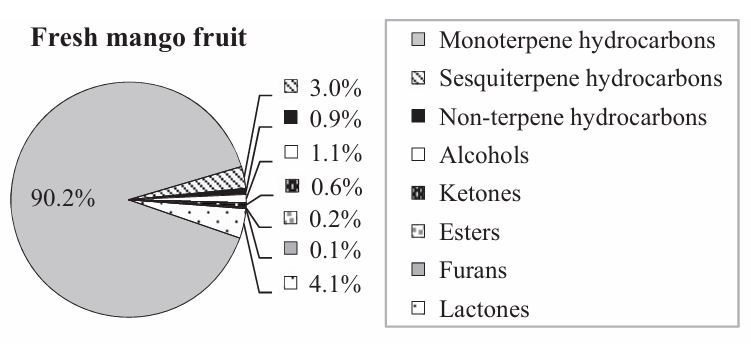
\includegraphics[width=0.8\textwidth]{Figures/fig_fresh_mango_chemical_classes.JPG}
    \caption{Distribution $[\%]$ of chemical classes of volatile compounds in fresh mango. Adapted from Bonneau et al. (2016) \cite*{A07_Bonneau2016}.}
    \label{fig:mango_aroma_compounds}
\end{figure}

\subsection{Key Aroma Compounds in Mango}
In this subsection, the key aroma compounds identified from fresh mango fruits in the study by Bonneau et al. (2016) are discussed \cite*{A07_Bonneau2016}. .

\subsubsection*{Terpenes and Terpenoids}
Terpenes represent the largest class of mango aroma compounds, derived from isoprene units via the terpenoid biosynthetic pathway \cite*{A09_Barras2024}. They include both monoterpenes and sesquiterpenes, which together account for the majority of mango volatiles \cite*{A07_Bonneau2016}. Terpenes and terpenoids are found in many different natural sources, including fruits, plants, animals, microbes, and fungi. The terpenes belong to the largest class of secondary metabolites in nature and consist of five connected carbon atoms, known as isoprene units. These carbon units can be assembled in thousands of ways \cite*{B01_TerpenesTerpenoids_2018}. The terpenoids are further subcualified into five sub-groups based on the number of isoprene units they contain: monoterpenes (C10), sesquiterpenes (C15), diterpenes (C20), sesterterpenes (C25), and triterpenes (C30) \cite*{B01_TerpenesTerpenoids_2018}.


\paragraph*{Monoterpene hydrocarbons}
A total of 11 monoterpene hydrocarbons were identified as key aroma compounds in fresh mango \cite*{A07_Bonneau2016}. The most significant ones include: $\alpha$-phellandrene, $\gamma$-terpinene, $\delta$-3-carnene, $\beta$-myrcene, $\alpha$-terpinene, limonene, $\beta$-phellandrene, and $\alpha$-terpineol. 

Monoterpenes are the smallest molecules in the isoprenoid family with conserved hydrocarbons \cite*{A09_Barras2024}. They share the formula $C_{10}H_{16}$ and over 400 different chemical structures has been classified as such \cite*{A09_Barras2024}. The key monoterpene hydrocarbons identified in mangos are reported to have significant impact on the overall odorants \cite*{A07_Bonneau2016}.

\paragraph*{Sesquiterpene hydrocarbons}
Compared to monoterpenes, sesquiterpenes are larger molecules with the formula $C_{15}H_{24}$. In mango fruit, the study by Bonneau et al. (2016) identified four key sesquiterpene hydrocarbons, including: $\alpha$-gurjunene, $\alpha$-copaene, $\beta$-caryophyllene, and $\alpha$-caryophyllene \cite*{A07_Bonneau2016}.

\subsubsection*{Alcohols and Aromatic Alcohols}
Alcohols and aromatic alcohols are, like terpenes and terpenoids, major contributors to the key aroma of mango, though they differ in chemical structure and biosynthetic origin. A study by Singh et al. (2010) highlighted the role of alcohol dehydrogenase (ADH) in the enzymatic reduction of aldehydes leading to the formation of these compounds \cite*{A10_Singh2010}.

\vspace{1em}
A total of nine alcohols were identified as key aroma compounds in fresh mango \cite*{A07_Bonneau2016}. The most significant ones include: 2-methyl-1-propanol, 1-pentanol, (\textit{E})-2-penten-1-ol, (\textit{Z})-2-penten-1-ol, 1-octanol, 1-butanol, 3-methyl-1-butanol, 2-decanol, 1-hexanol, and (\textit{Z})-3-hexen-1-ol \cite*{A07_Bonneau2016}.

\subsubsection*{Aldehydes and Aromatic Aldehydes}
Aldehydes are volatile compounds primarily formed through the oxidation of unsaturated fatty acids, such as $\alpha$-linolenic acid, via the lipoxygenase (LOX)-hydroperoxide lyase (HPL) pathway. These reactions generate C$_6$ and C$_9$ aldehydes, often referred to as green leaf volatiles, which are associated with fresh and grassy notes in the mango fruit aroma \cite*{A11_Sivankalyani2017}. In mango, this pathway becomes particularly active under chilling stress, leading to increased levels of compounds such as 1-hexanal, (\textit{E})-2-hexenal, and (\textit{Z})-3-hexenal before visible quality loss occurs.

\vspace{1em}
In fresh mango, a total of six aldehydes were identified as key aroma compounds \cite*{A07_Bonneau2016}. The most significant ones include hexanal, (\textit{E,E})-2,4-heptadienal, nonanal, and (\textit{E,Z})-2,4-heptadienal \cite*{A07_Bonneau2016}.

\subsubsection*{Lactones}
Lactones are VOCs that quantitatively represents a smaller fraction of the mango aroma profile compared to terpenes and terpenoids. They are nonetheless important contributors to the overall sensory experience of the fruit, and make up two times the quantitative amount of alcohols, ketones, esters, and furans combined \cite*{A14_Silva2021, A07_Bonneau2016}. Lactones are cyclic esters formed through the intramolecular esterification of hydroxy acids. In mango, they are primarily derived from the oxidation and subsequent cyclization of fatty acids during the ripening process \cite*{A13_ElHadi2013}.

\vspace{1em}
A total of five lactones were identified as key aroma compounds in fresh mango, in the study by \textcite*{A07_Bonneau2016}. The most significant ones include: $\alpha$-methyl-$\gamma$-bytyrolactone, $\gamma$-hexalactone, $\delta$-hexalactone, and $\delta$-ocatlacetone \cite*{A07_Bonneau2016}.

\subsubsection*{Minor Volatile Compounds: Ketones, Esters, and Furans}
Ketones, esters, and furans are present in much smaller amounts compared to terpenes and terpenoids, but still contribute to the complexity of mango aroma \cite*{A07_Bonneau2016}. Ketones can arise from the enzymatic reduction of carbonyl compounds, as demonstrated by bioreduction studies on tropical fruit tissues \cite*{A12_Lemos2008}. Esters are associated with fruity and sweet nuances, whereas the furans provide the mango fruit with mild caramel-like notes. Despite low abundance of these three classes of compounds, they may enhance the overall balance of aroma perception in fresh mango \cite*{A13_ElHadi2013}.

\subsection{Variation in Aroma Profiles Among Mango Varieties}
The volatile composition of mango (\textit{Mangifera indica} L.) varies substantially among cultivars, reflecting genetic differences and environmental influences on fruit metabolism and ripening \cite*{A01_Aguirre-Lopez_2023}. Comparative analyses of multiple mango varieties has shown that the abundance and composition of key aroma compounds differ significantly across cultivars, leading to distinct sensory profiles \cite*{A01_Aguirre-Lopez_2023,A02_Moreno2010}. 

\vspace{1em}
A recent study by \textcite{A16_Tandel2023} investigated 16 different Indian mango cultivars, revealing significant differences in their volatile profiles \cite*{A16_Tandel2023}. Cultivars such as \textit{Alphonso}, \textit{Kesar}, and \textit{Ratna}, were characterised by their high levels of terpenes, whereas the variety \textit{Amrapali} was the dominant in esters \cite*{A16_Tandel2023}. The cultivar \textit{Kesar} exhibited the highest content of monoterpenes, showcasing a total of 91.00\%, while two other cultivars, \textit{Dashehari} and \textit{Neelum} had 0.00\% monoterpenes \cite*{A16_Tandel2023}. Instead, the \textit{Dashehari} cultivar were rich in sesquiterpenes and fatty acids, showing a total of 23.76\% and 37.91\%, respectively \cite*{A16_Tandel2023}.

Within the terpene class, \textit{allo-ociemene} was the dominant monterpene across most cultivars, with a concentration ranging from 4.99\% in \textit{Neeleswari} to 89.36\% in \textit{Sonpari} \cite*{A16_Tandel2023}. The cultivar \textit{Amrapali} stood out with a high ester content of 18.49\%, primarily due to the presence of butanoic acid \cite*{A16_Tandel2023}.

\vspace{1em}
A study by \textcite{A13_ElHadi2013} further distinguished the aroma profiles of different mango cultivars according to their geographical origin \cite*{A13_ElHadi2013}. New Worlds varieties, e.g. \textit{Haden}, \textit{Irwin}, \textit{Manila}, and \textit{Tommy Atkins}, were typically dominated by terpene hydrocarbons—especially $\delta$-3-carene. 

Especially 3-carene was a dominant compound in New World mangoes, and constituted 16-90\% of total volatiles, followed by  $\alpha$-pinene, $\alpha$-phellandrene, and $\sigma$-3-carene \cite*{A13_ElHadi2013}. In contrast, Old World varieties tended to exhibit higher proportions of esters, alcohols, and ketones, resulting in sweeter and fruitier aroma profiles \cite*{A13_ElHadi2013}, althrough, \textcite{A13_ElHadi2013} reported a larger difference in VOC quantity and quality in Old World cultivars compared to New World ones \cite*{A13_ElHadi2013}. 

\vspace{1em}
As discussed by \textcite{A16_Tandel2023}, previous studies have compared two Chinese mango cultivars, \textit{Tainong} and \textit{Jinmang}, which exhibited high levels of $\beta$-ocimene, myrcene, and $\alpha$-terpinolene, which significantly contributed to their aroma profiles. These observations align with the findings of \textcite{A15_Xie2023}, who also reported terpenes as being a dominant volatile class in the Chinese cultivar \textit{Jinmang} \cite*{A16_Tandel2023, A15_Xie2023}.


\vspace{1em}
\textcite{A15_Xie2023} conducted a detailed comparison between the Chinese cultivars \textit{Tainong} and \textit{Hongyu}, revealing cultivar-specific differences in their volatile composition \cite*{A15_Xie2023}. The \textit{Tainong} mango contained a higher concentration of terpenes and aldehydes, thereby producing a characteristic grassy aroma.  In contrast, the \textit{Hongyu} exhibited higher ester levels, contributing to a more fruity and sweet aroma \cite*{A15_Xie2023}. Key distinguishing VOCs included $\beta$-ocimene for the terpene-lemon profile of \textit{Tainong} and propyl butyrate for the fruity character of \textit{Hongyu} \cite*{A15_Xie2023}.



\section{Biochemical Pathways of Aroma Compound Formation}
VOCs are low-molecular-weight molecules encompassing diverse functional groups such as alcohols, esters, ketones, aldehydes, and terpenes \cite*{A01_Aguirre-Lopez_2023, B01_TerpenesTerpenoids_2018}. In fruits, VOCs are released through metabolic and enzymatic reactions during maturation and ripening, consolidating the fruit’s characteristic aroma potential \cite*{A01_Aguirre-Lopez_2023}. VOC profiling is therefore essential for characterizing varieties, assessing quality, and determining ripeness. The aromatic profile of mango is composed of aldehydes (24.2\%), alcohols (16.5\%), esters (34.0\%), and other compounds including terpenes, ketones, furans, lactones, and sulfur volatiles (25.3\%) \cite*{A01_Aguirre-Lopez_2023}.

\vspace{1em}
Understanding the formation of these compounds requires examination of the biochemical mechanisms underlying their production. The field of \textit{volatilomics} investigates the biogenesis and metabolic routes of aroma compounds \cite*{A01_Aguirre-Lopez_2023}. The main precursor substrates are amino acids, fatty acids, and carbohydrate- or terpenoid-derived intermediates \cite*{A13_ElHadi2013}. Once the basic skeletons are formed, further enzymatic transformations such as hydroxylation, acylation, methylation, oxidation–reduction, and ring closure increase molecular diversity and volatility. The following subsections will explore these pathways—namely the Terpenoid Pathway (MVA and MEP), the Fatty Acid Derivative Pathway, and the Amino Acid Derivative Pathway—as well as the specific enzymes, such as alcohol dehydrogenases (ADH), that drive these reactions during fruit development \cite*{A10_Singh2010}.

%VOCs are low molecular weight molecules present in biological systems, encompassing diverse functional groups such as alcohols, esters, ketones, aldehydes, and terpenes \cite*{A01_Aguirre-Lopez_2023, B01_TerpenesTerpenoids_2018}. These compounds are naturally released by organisms as a product of biogenic processes \cite*{A01_Aguirre-Lopez_2023}. In fruits, VOCs are crucial substances liberated during the biochemical processes of maturation and ripening, which involve underlying metabolic activity and enzymatic hydrolysis that consolidate the fruit's characteristic aroma potential \cite*{A01_Aguirre-Lopez_2023}. Consequently, VOC analysis is essential for characterizing varieties, assessing quality, and determining the fruit's state of maturity \cite*{A01_Aguirre-Lopez_2023}. The resultant complex aromatic profile is composed of major chemical classes, including aldehydes (24.2\%), alcohols (16.5\%), esters (34.0\%), and other compounds like terpenes, ketones, furans, lactones, and sulfur compounds (25.3\%) \cite*{A01_Aguirre-Lopez_2023}.

\vspace{1em}
%Understanding the generation of this chemical complexity requires examination of the mechanisms underlying their formation, a field of study referred to as volatilomics, which seeks to comprehend the biogenesis of aromatic compounds and define the metabolic routes from which they proceed \cite*{A01_Aguirre-Lopez_2023}. The diversity of these volatile substances arises from several major biosynthetic pathways that convert primary precursor substrates into volatile products \cite*{A13_ElHadi2013}. These precursors include amino acids, membrane lipids/fatty acids, and compounds derived from carbohydrates/terpenoids \cite*{A13_ElHadi2013}. Once the basic chemical skeletons are synthesized through these primary routes, the final aroma compounds are diversified through additional enzymatic modification reactions, such as hydroxylation, acylation, methylation, oxidation/reduction, and cyclic ring closure, increasing their volatility and complexity \cite*{A13_ElHadi2013}. The following subsections will explore these critical pathways—namely the Terpenoid Pathway (MVA and MEP), the Fatty Acid Derivative Pathway, and the Amino Acid Derivative Pathway—as well as the specific enzymes, such as alcohol dehydrogenases (ADH), that are central to driving these flavor-forming reactions during fruit development \cite*{A10_Singh2010}.

\subsection{Overview of Biosynthetic Pathways}

\subsection{Enzymes Involved in Aroma Biosynthesis}

\subsection{Terpenoid Pathway (MEP and MVA Pathways)}

\subsection{Fatty Acid Derivative Pathway}

\subsection{Amino Acid Derivative Pathway}


\section{Environmental and Genetic Factors Influencing Aroma Production}
\subsection{Pre-harvest Factors}
\subsection{Post-harvest Factors}
\subsection{Processing Implications on Aroma Retention}


\section{Analytical Techniques for Aroma Compound Identification}
\subsection{Extraction and Analysis Methods}
\subsection{Quantification and Sensory Evaluation}

\section{Comparative Perspective}

\section{Conclusion}
